\documentclass{scrartcl}
\usepackage{threeparttable}

\usepackage{relsize}
\usepackage{xspace}

\usepackage{listings}
\lstset{language=MATLAB,numbers=left,frame=lines}
\lstnewenvironment{snippet}{\lstset{numbers=none,frame=none}}{}

\usepackage{amsmath}
\usepackage{amsfonts}

\usepackage{graphicx}

\usepackage{tikz}
\usetikzlibrary{shapes,arrows}
\tikzstyle{decision} = [diamond, draw, fill=blue!20, 
    text width=4.5em, text badly centered, node distance=3cm, inner sep=0pt]
\tikzstyle{block} = [rectangle, draw, fill=blue!20, 
    text width=7em, text centered, rounded corners, minimum height=4em]
\tikzstyle{line} = [draw, -latex']
\tikzstyle{cloud} = [draw, ellipse,fill=red!20, node distance=3cm,
    minimum height=2em]


\newcommand{\RR}{\mathbb{R}}
\newcommand{\trace}{\textrm{tr}}
\renewcommand{\SS}{\mathbb{S}}

\newcommand{\find}{\textrm{find}}
\newcommand{\minimize}{\textrm{minimize}}
\newcommand{\maximize}{\textrm{maximize}}
\newcommand{\subjto}{\textrm{subj. to}}

\newcommand{\li}[1]{\lstinline{#1}}
\newcommand{\spotless}{SPOT{\relsize{-2}LESS}\xspace}
\newcommand{\msspoly}{\lstinline{ msspoly}\xspace}
\newcommand{\spotprog}{\lstinline{spotprog}\xspace}
\newcommand{\spotsdpsol}{\lstinline{spotsdpsol}\xspace}
\newcommand{\spotsosprog}{\lstinline{spotsosprog}\xspace}




%\newcommand{\matlab}{MATLAB$^\textregistered$}
\title{\spotless \\ Polynomial and Conic Optimization}
\author{ Mark M. Tobenkin, Frank Permenter, Alexandre Megretski}
\begin{document}
\maketitle
\tableofcontents
\section{Introduction}
\spotless is a software toolbox for MATLAB for posting conic \cite{cone} and sum-of-squares (SOS) optimization problems \cite{sos}.
The basic functionality provided:
\begin{enumerate}
\item A simple, reasonably fast approximate symbolic algebra package.
\item A modeling tool for posing and pre-/post-processing conic optimization problems.
\item A modeling tool for posing SOS problems.
\end{enumerate}
Several alternative tools exist for addressing these problems, notably  CVX \cite{cvx} and Yalmip \cite{yalmip}.  We recommend these packages as more user-friendly modeling environments -- the emphasis of \spotless is on providing an {\it extensible} tool for {\it  building other libraries}.





\section{Quick Start}
This section provides an explanation of the basic capabilities of \spotless, and provides simple examples of solving conic and SOS programs and inspecting the solutions.

\subsection{Basic \spotless Work-Flow}
The basic work-flow in \spotless is as described by Figure~\ref{fig:basic}.

\begin{figure}
  \centering
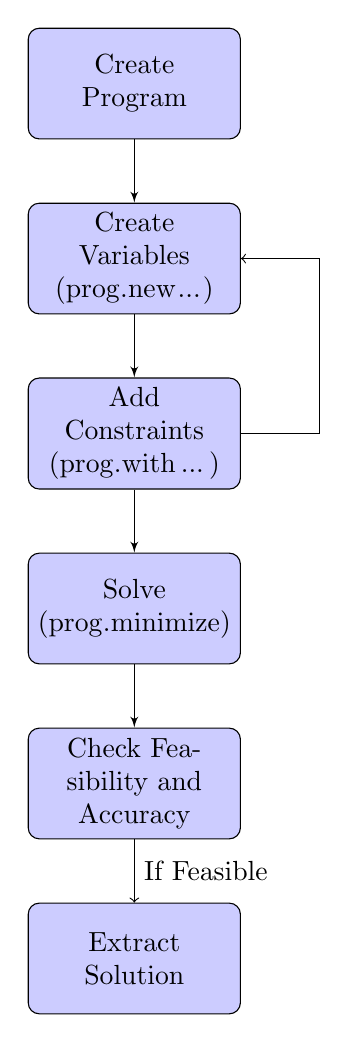
\begin{tikzpicture}[node distance = 2.222222cm, auto]
    % Place nodes
    \node [block] (prog) {Create \\Program};
    \node [block,below of=prog] (new) {Create \\ Variables\\(\lstinline{prog.new...})};
    \node [block,below of=new] (with) {Add \\Constraints\\ (\lstinline{prog.with...})};
    \node [block,below of=with] (solve) {Solve \\ (\lstinline{prog.minimize})};
    \node [block,below of=solve] (feas) {Check Feasibility and Accuracy};
    \node [block,below of=feas] (solution) {Extract Solution};

    \path[line] (prog) -- (new);
    \path[line] (new) -- (with);
    \path[line] (solve) -- (feas);
    \draw[->] (feas) -- node[pos=0.5]{If Feasible}(solution);
    \draw [->]  (with.east)  -- ++(10mm,0) |- node [black, near end, yshift=0.75em] {} (new.east);    
    \path[line] (with) -- (solve);
  \end{tikzpicture}
\caption{Basic \spotless workflow.\label{fig:basic}}
\end{figure}

Let's walk through the following example to provide some more detail.
The input to the program is a pair of positive integers $(n,m)$ a matrix $A \in \RR^{n \times m}$ and a vector $b \in \RR^{n}$. The program is defined by:
\begin{flalign*}
  \mathop{\minimize}_{x\in\RR^m} \quad & \sum_{i=1}^m |x_i|\\
  \subjto \quad & Ax = b.
\end{flalign*}
\begin{lstlisting}
prog = spotprog;
[prog,x] = prog.newFree(m);
prog = prog.withEqs(A*x - b);

[prog,a] = prog.newPos(m);
prog = prog.withPos(a - x);
prog = prog.withPos(a - (-x));

obj = sum(a);

sol = prog.minimize(obj);

if sol.solutionQuality < 0
    error('Solution is of very low quality.');
elseif sol.solutionQuality < 1
    warning('Low solution quality.');
end
if sol.primalInfeasible || sol.dualInfeasible
    error('Infeasibility detected.');
end

xopt = double(sol.eval(x));
\end{lstlisting}

\subsubsection{Create a program} First, one constructs a program object as in
\begin{lstlisting}[firstnumber=1,frame=none]
  prog = spotprog;
\end{lstlisting}
for conic programming. For SOS programming one instead uses
\begin{lstlisting}[numbers=none,frame=none]
  prog = spotsosprog;
\end{lstlisting}
\subsubsection{Create Variables}
  Next, one constructs new decision variables, e.g.
\begin{lstlisting}[frame=none,firstnumber=2]
[prog,x] = prog.newFree(m);
\end{lstlisting}
updates \lstinline{prog} to have \li{m} new free (unconstrained) variables, stored in the vector \li{x}.
A similar syntax modifies the program to have \li{m} non-negative variables:
as in
\begin{lstlisting}[frame=none,firstnumber=5]
[prog,a] = prog.newPos(m);
\end{lstlisting}
stored in the vector \li{a}.  The types supported by \spotprog are  listed in Table~\ref{tab:spotprog_types}.  
\subsubsection{Add Constraints}
  Equality constraints are defined by expressions which must be equal to zero, i.e.
\begin{lstlisting}[frame=none,firstnumber=3]
prog = prog.withEqs(A*x - b);
\end{lstlisting}
ensures $Ax = b$.  Additional ``conic'' constraints can be added, e.g.
\begin{lstlisting}[frame=none,firstnumber=6]
prog = prog.withPos(a - x);
\end{lstlisting}
  requires \lstinline{a(i)} $\geq$ \lstinline{x(i)} for $i \in \{1,\ldots,m\}$.
  Similar function calls, (i.e. \lstinline{prog.withType()}) are used to impose other kinds of constraints.
\subsubsection{Solve The Program}
The next step is to identify an objective, and solve the program:
\begin{lstlisting}[frame=none,firstnumber=11]
sol = prog.minimize(obj);
\end{lstlisting}
here \li{obj} is an affine expression in decision parameters and \li{sol} is a solution object.
Calling \li{prog.minimize} without a first argument, or with zero as the first argument solves a feasibility problem.  See Section~\ref{sec:sol} for more details about specifying a solver and adding pre-/post-processing options.
\subsubsection{Examine Feasibility and Accuracy}
Ideally, a ``solution'' to a conic programming problem should consist of one of:
\begin{enumerate}
  \item[(i)] A pair of primal and dual feasible points which are optimal.
  \item[(ii)] A primal improving direction (proving dual infeasibility).
  \item[(iii)] A dual improving direction (proving primal infeasibility).
\end{enumerate}
Solution {\it quality} in \spotless refers to a numerical measure of confidence that the solver has obtained such a solution.
Both poorly posed problems and numerical errors can lead to a low quality solution.
Section~\ref{sec:bad} contains some examples of programs for which no solution in the above sense exists.

Once a solver has been called, one must examine the quality of the returned solution. Note that {\bf the interpretation of solution quality is application dependent!}  Please see Section~\ref{sec:sol} for information about customizing solution quality reporting for your application.  
Negative solution quality is supposed to indicate a useless solution, as tested by
\begin{lstlisting}[frame=none,firstnumber=13]
if sol.solutionQuality < 0
\end{lstlisting}
whereas solution quality less than \li{1} is supposed to be circumspect.

If the soluton quality is high, one can still have an {\it infeasible} program, as test by
\begin{lstlisting}[frame=none,firstnumber=18]
if sol.primalInfeasible || sol.dualInfeasible
\end{lstlisting}
Primal infeasibility generally implies that no choice of decision variables satisfies the given constraints.  Dual infeasibility often means that the optimal cost is unbounded below.  A more thorough account is given in Section~\ref{sec:feas}.
\subsubsection{Extract Solution}
To extract a solution, one first uses \li{sol.eval} to substitute optimal decision parameters into any algebraic expression, e.g.
\begin{lstlisting}[frame=none,firstnumber=18]
xopt = double(sol.eval(x));
\end{lstlisting}
Here, \li{double} is then used to transform the resulting expression from \spotless's internal symbolic algebra library into a numerical vector.
\subsection{Basic Types}


\begin{table}
  \centering
  \begin{threeparttable}[b]
  \caption{Constraint Types for \spotprog\label{tab:spotprog_types}}
  \begin{tabular}{|l|lll|}
    \hline
    Type& Abbrev. & Vector Space & Constraint\\
    \hline
    Free & \lstinline!Free! & $ x \in \RR^n$ & \\
    Positive & \lstinline!Pos! & $x\in\RR^n$ & $x_i \geq 0$\\
    Lorentz & \lstinline!Lor! & $x \in\RR^{n\times m}$ & $x_{1j}^2 \geq \sum_{i=2}^n |x_{ij}|^2$, \quad $\forall j$\\
    Rotated Lorentz & \lstinline!RLor! & $x\in\RR^{n\times m}$ & $x_{1j} \geq 0, \quad x_{1j}x_{2j} \geq \sum_{i=3}^n |x_{ij}|^2$\quad $\forall j$\\
    Positive Semidefinite & \lstinline!PSD! & See below.\tnote{1}
&\\
\hline
\end{tabular}
\begin{tablenotes}
\item [1]  The positive semidefinite cone refers to matrices $X \in \RR^{n\times n}$ such that $v^T X v \geq 0$
      for all $v \in \RR^n$.  Two representations are used in \spotless:  a single PSD variable can be represented by an $n\times n$ \msspoly and  a set of $N$ PSD variables can be represented as ${n+1 \choose 2}\times N$ \msspoly.  When $N=1$ this transformation from one representation to the other is given by \lstinline{mss_v2s} (read: vector-to-symmetric) and \lstinline{mss_s2v} (read: symmetric-to-vector):
  \[
  \lstinline{mss_s2v(X)} = \begin{bmatrix} X_{11} \\ X_{12} \\ X_{22} \\ X_{13} \\ \vdots\end{bmatrix}
\qquad   \lstinline{mss_v2s(x)} = \begin{bmatrix}
    x_1 & x_2 & x_4 & \ldots \\
    x_2 & x_3 & x_5 & \ldots \\
    x_5 & x_3 & x_6 & \ldots \\
    \vdots & \vdots & \vdots & \ddots
  \end{bmatrix},
  \]
  where $X \in \RR^{n\times n}$ and $x \in \RR^{n+1 \choose 2}$.
  {\bf N.B.}: Generally:
  \[
 \trace(\lstinline[mathescape]!X*S!) \not \equiv \lstinline{mss_s2v}(X)'*\lstinline{mss_s2v}(S).
 \]
\end{tablenotes}
\end{threeparttable}
\end{table}

% \end{tabular}



\subsection{Conic Programming Examples}
\subsubsection{$\ell_\infty$ Fitting Example}
Given an positive integers $N$ and $d$ find $x \in \RR^{n}$ to solve:
\begin{flalign*}
  \minimize \quad & \max_{i \in \{-N,\ldots,N\}} \left \{\left |\sum_{i=0}^d x_{i+1} \left(\frac{i}{N}\right)^d - \left |\frac{i}{N}\right|\right| \right \}, \\
  \subjto \quad & x \in \RR^{d+1}.
\end{flalign*}
\lstinputlisting[title=examples/linf\_fitting.m]{examples/linf_fitting.m}
This program fits a degree 5 polynomial in $t$ to the function $|t|$ over $[-1,1]$.  Line 9 constructs a new program.  Lines 11 and 12 introduce the indeterminate t and constructs the vector \lstinline{basis = [ 1 ; t ; ... ; t^d]}.  A vector of $d+1$ coefficients are created on Line 13, and on Line 14 used to construct a function \lstinline{f = coeff(1) + coeff(2)t + ...}.  The function \lstinline{msubs} is used on line 16 to evaluate \lstinline{f} at each \lstinline{t = tt(i)} (returning a row).  Finally Lines 19 and 20 require the free variable \lstinline{obj} to satisfy \lstinline{obj} $\geq$ \lstinline{err(i)} and \lstinline{-err(i)}  respectively for each $i$.  The program is solved (Line 22), and the optimal coefficients are substituted into \lstinline{f} and stored in \lstinline{fopt} on Line 24.

\subsubsection{SDP Projection Example}
Given $A = A' \in \RR^{n\times n}$, solve:
\begin{flalign*}
  \minimize \quad & \|A-X\|_F \\
  \subjto \quad & X \in \SS_{n,+}.
\end{flalign*}
\lstinputlisting[title=examples/sdp\_projection.m]{examples/sdp_projection.m}

The optimization problem begins at line 6 by constructing a new program.  Line 7 constructs a new $n\times n$ PSD decision variable,\lstinline{P}, and line 8 a 1-by-1 free variable, \lstinline{obj}.  Line 10 constraints \lstinline{obj} to be greater than the $2$-norm of $P-A$ when regarded of as a vector using a Lorentz cone constraint (see Section \ref{sec:cones}).  A solution is then generated to the problem of minimizing \lstinline{obj} with the default solver on Line 12.  Finally, Line 14 substitutes the optimizing variables into the expression for \lstinline{P}, and then transforms that expression in a MATLAB double array stored in \lstinline{Popt}.


\subsubsection{SDP Control Design Example}
Given a matrix pair $(A,B) \in \RR^{n\times n} \times \RR^{n \times m}$ representing a stabilizable discrete time LTI system
\[
x[t+1] = A x[t] + B u[t],
\]
find matrix $K \in \RR^{m \times n}$ such that $A+BK$ is exponentially stable.
For $\rho \in (0,1)$ solve
\begin{flalign*}
  \find \quad & (S,L) \in \SS_{n,+} \times \RR^{m\times n} \\
  \subjto \quad & 
\begin{bmatrix} (1-\rho)S   & AS+BL\\
  SA'+L'B' &   S
  \end{bmatrix} \in \SS_{2n,+}.
\end{flalign*}
and take $K = LS^{-1}$.
\lstinputlisting[title=examples/sdp\_lti\_control.m]{examples/sdp_lti_control.m}



\subsection{SOS Programming Examples}
\subsubsection{Upper Bound Polynomial On Sphere}
\begin{lstlisting}
% Construct a random polynomial.
n = 2;
d = 4;
x = msspoly('x',n);
basis = monomials(x,0:d);
p = randn(length(basis))'*basis;

g = 1 - x'*x;

prog = spotsosprog;
prog = prog.withIndeterminate(x);
[prog,r] = prog.newFree(1);

[prog,f] = prog.newFreePoly(x,monomials(x,0:d-2));
prog = prog.withSOS(r-p-f*g);

sol = prog.minimize(r);

sol.eval(r);
\end{lstlisting}
\subsubsection{Van der Pol ROA}
\subsubsection{Simple Pendulum ROA}




\section{Basic Classes}
\subsection{\msspoly: Simple Approximate Symbolic Algebra}
\subsection{\spotprog: Representation of Optimization Problems}
\subsection{\spotsdpsol: Representation of Optimization Solutions}
\subsection{\spotsosprog: Representation of SOS Problems}
\section{Function Guide}
\end{document}